\chapter{Materials and Methods}

\section{Datasets}

The dataset utilized in this study was provided by the supervisor and obtained by the company Ornavera. Ornavera is dedicated to generating actionable data insights for agricultural health. Their mission is to create tools for data collection in agriculture, automating mathematical and scientific processes to benefit farmers through artificial intelligence and precision agriculture.

\subsection{ORNAVERA Data Collection Device (DCD)}

The DCD is responsible for gathering and transmitting data from various geo-physical and plant sensors to the Ornavera Data Aggregation Device (DAD) using a certified LoRa® radio interface.
\begin{figure}[htbp]
    \centering
    \includegraphics[width=6 cm]{4_ChapterMaterials/figuras/DCDornavera.pdf}
    \caption{ORNAVERA Data Collection Device (DCD)\cite{ornavera2020dcd}}
    \LABFIG{FIG}
    \end{figure}

It features:
\begin{itemize}
    \item \textbf{Wireless Interface:} Utilizes LoRa® technology for long-range, low-power communication with a coverage radius of up to 15 km in rural areas and 5 km in urban areas.
    \item \textbf{Controller:} Equipped with a high-performance ARM® Cortex® microcontroller for efficient data handling and communication.
    \item \textbf{Power Supply:} Operates on a solar-assisted Li-ion battery with a backup life of 1-2 months depending on sensor usage.
    \item \textbf{Interfaces:} Supports multiple I2C, SPI, and RS485 connections for various sensors, with additional ports for future expansion.
    \item \textbf{Environmental Tolerance:} Designed to operate within a temperature range of -10°C to 55°C and humidity levels of 10\%-95\% RH.
\end{itemize}


The ORNAVERA Data Collection Device (DCD) is equipped with the following sensors:
\begin{itemize}
    \item \textbf{Temperature and Humidity Probe:} SHT20 from Sensirion, providing accurate measurements of ambient conditions around the pepper plant.
    \begin{figure}[htbp]
        \centering
        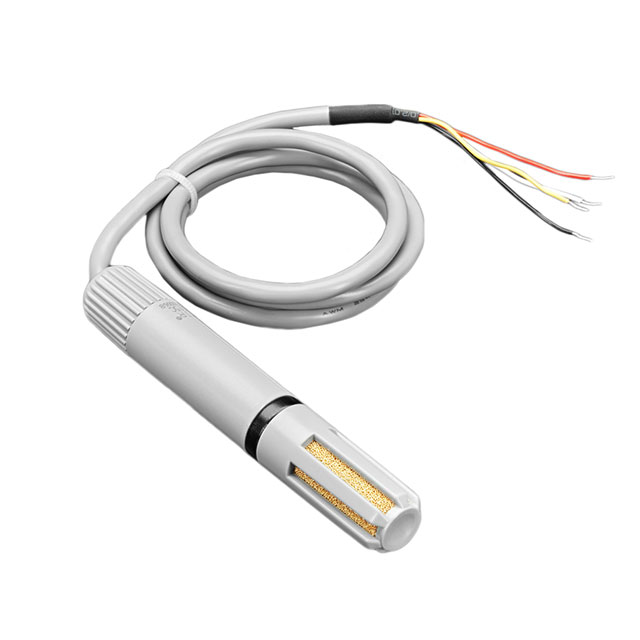
\includegraphics[width=6 cm]{4_ChapterMaterials/figuras/SHT20.jpg}
        \caption{Temperature and Humidity Probe: SHT20 from Sensirion\cite{ornavera2020dcd}}
        \LABFIG{FIG}
        \end{figure}

    \item \textbf{Soil Probe:} MEC-10, measuring soil moisture, pH, and other critical parameters for assessing soil health and suitability for pepper cultivation.
    \begin{figure}[htbp]
        \centering
        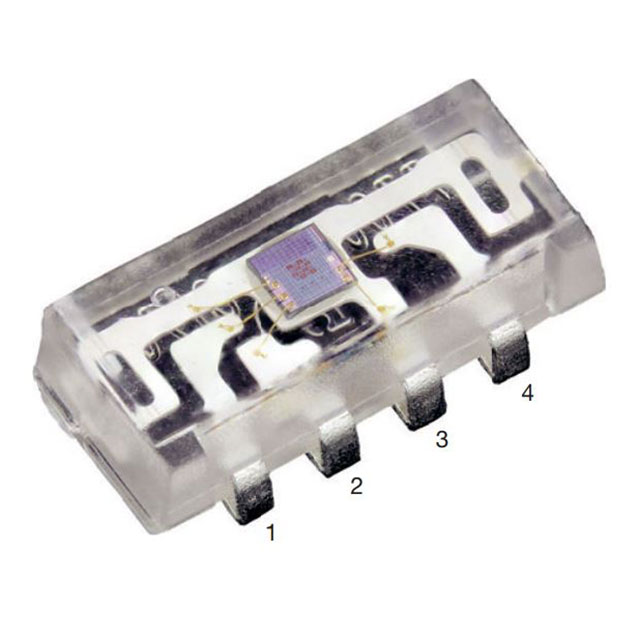
\includegraphics[width=6 cm]{4_ChapterMaterials/figuras/VEML7700.jpeg}
        \caption{Soil Probe: MEC-10 from Dalian Endeavour Technology Co. \cite{ornavera2020dcd}}
        \LABFIG{FIG}
        \end{figure}

    \item \textbf{Light Sensor:} VEML7700 from Vishay, used to measure light intensity impacting the pepper plant.
    \begin{figure}[htbp]
        \centering
        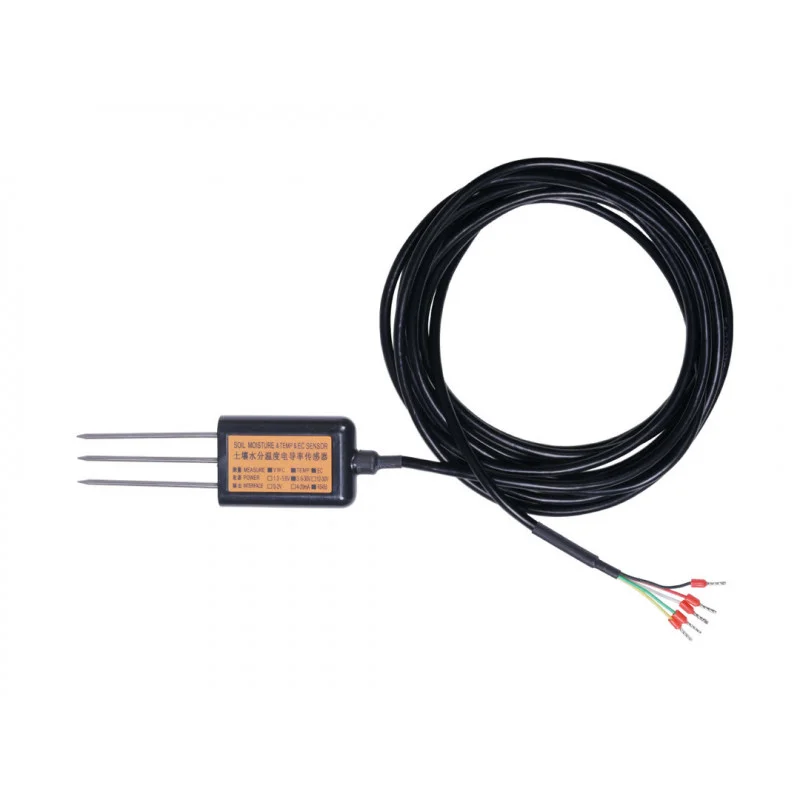
\includegraphics[width=6 cm]{4_ChapterMaterials/figuras/MEC10.png}
        \caption{Light Sensor: VEML7700 from Vishay.\cite{ornavera2020dcd}}
        \LABFIG{FIG}
        \end{figure}

    \item \textbf{Dendrometer:} Designed by Ornavera, used to measure the diameter of the pepper plant, essential for tracking its growth.
\end{itemize}


These sensors, integrated with the DCD, provided a detailed dataset for analyzing the environmental and soil conditions affecting pepper plant growth. The data collected was carefully recorded and analyzed to draw valuable insights for the study.


\section{Available Variables}

Thanks to the sensors mentioned previously, we have been able to extract a set of crucial variables for analyzing the growth of pepper plants. These data allow us to accurately assess the environmental and soil conditions that influence plant development. In the following section, the importance of these variables in plant growth is explained, highlighting how each one contributes to a better understanding of the agricultural environment and the optimization of cultivation practices.

\subsection{Temperature (t1)}

Temperature is a fundamental factor influencing plant growth, as it affects critical physiological processes such as photosynthesis, respiration, and transpiration. The variable \( t1 \) measures the ambient air temperature surrounding the plant, which is essential for determining whether environmental conditions are conducive to optimal growth. For instance, most plants have a specific temperature range within which they perform best. Outside this range, physiological processes can become less efficient, potentially leading to stress. For example, excessively high temperatures can increase respiration rates to the detriment of photosynthesis, ultimately hindering plant growth. Conversely, low temperatures can slow down metabolic activities, leading to reduced growth rates. Therefore, maintaining optimal temperature conditions can enhance the overall productivity and health of plants, making it a crucial variable to monitor.

\subsection{Relative Humidity (rh1)}

Relative humidity (\( rh1 \)) is another critical environmental factor, representing the percentage of moisture in the air relative to the maximum amount the air can hold at a given temperature. It plays a significant role in plant water use efficiency and disease management. High relative humidity can reduce transpiration rates, which might lead to an accumulation of water in the plant and potentially create conditions for disease, particularly fungal infections. Conversely, low humidity levels can cause increased transpiration, leading to water stress if not balanced by sufficient water uptake from the soil. Properly managing humidity levels is crucial for optimizing plant health, as it impacts everything from water uptake to disease resistance. Understanding relative humidity patterns allows farmers to adjust irrigation practices and greenhouse conditions to improve crop resilience and productivity.

\subsection{Vapor Pressure Deficit (vpd1)}

Vapor Pressure Deficit (VPD), derived from relative humidity and temperature, provides insights into the drying power of the air. It represents the difference between the amount of moisture in the air and how much moisture the air can hold when saturated. This measure is crucial for understanding plant transpiration rates and water stress levels. High VPD indicates drier air, which can increase transpiration and potentially lead to water stress if not adequately managed. On the other hand, low VPD suggests more humid conditions, which can reduce transpiration and, in some cases, lead to an excess of moisture around the plant, fostering mold and mildew. By monitoring VPD, growers can make informed decisions about irrigation and climate control, ensuring plants receive the optimal balance of moisture to thrive.

\subsection{Light Intensity (lux)}

Light intensity, measured in lumens (lux), is crucial for plant growth as it directly impacts photosynthesis—the process by which plants convert light into energy. Adequate light intensity is essential for driving this process, influencing growth rates and overall plant health. Insufficient light can limit photosynthesis, stunting growth and leading to weaker plants, while excessive light can cause photoinhibition, where too much light actually damages the photosynthetic apparatus, reducing efficiency. Understanding and managing light exposure is therefore vital for maximizing photosynthetic activity, especially in controlled environments like greenhouses. By ensuring that plants receive the right amount of light, farmers can enhance growth rates, improve flowering and fruiting patterns, and optimize crop yields.

\subsection{Soil Temperature (st1)}

Soil temperature (\( st1 \)) is a key variable that influences root activity and microbial processes in the soil, both of which are critical for nutrient uptake and plant growth. Soil temperature affects root metabolism, with optimal temperatures promoting vigorous root growth and nutrient absorption. If soil temperatures fall outside the optimal range, root activity can slow down, impairing the plant's ability to access water and nutrients, and potentially leading to stunted growth. Additionally, soil temperature affects the activity of soil microbes, which play a vital role in decomposing organic matter and releasing nutrients in forms that plants can absorb. Monitoring soil temperature helps in managing planting schedules and optimizing root zone conditions to ensure that plants have access to the nutrients they need for healthy growth and development.

\subsection{Permittivity (p1)}

Permittivity is a measure of a soil's ability to store and transmit electric fields, closely related to its moisture content. High permittivity often indicates a higher soil moisture level, which is crucial for nutrient transport and root uptake. Adequate soil moisture facilitates the movement of nutrients from the soil to the plant roots, thereby supporting healthy growth. However, too much moisture can lead to waterlogged conditions, which can suffocate roots and inhibit their ability to function properly. By measuring permittivity, growers can gain insights into soil moisture levels and make informed decisions about irrigation practices. This ensures that plants receive the optimal amount of water, reducing stress and enhancing growth conditions, which is particularly important for maintaining crop health in varying weather conditions.

\subsection{Electrical Conductivity (ec1)}

Electrical conductivity (\( ec1 \)) measures the soil's ability to conduct electricity, which is indicative of the concentration of soluble salts and nutrients in the soil. High electrical conductivity can indicate excessive salts, which may lead to osmotic stress and interfere with nutrient uptake. This can harm plant growth, especially in crops sensitive to salinity. On the other hand, low electrical conductivity may suggest nutrient deficiencies that can limit growth and yield. Monitoring electrical conductivity is essential for diagnosing soil fertility and salinity issues, allowing farmers to adjust fertilization practices accordingly. By maintaining balanced nutrient levels, plants can achieve optimal growth and productivity, highlighting the importance of regular soil EC monitoring.

\subsection{Volumetric Water Content (vwc1)}

Volumetric Water Content (\( vwc1 \)) measures the percentage of water present in the soil, reflecting the soil moisture status and availability for plant uptake. This variable is crucial for understanding the water dynamics within the soil and ensuring plants have sufficient water for physiological processes. Adequate soil moisture supports nutrient uptake and maintains plant turgor, which is vital for growth and stability. However, both insufficient and excessive moisture can cause stress: too little water can lead to drought stress, while too much can lead to root rot and decreased oxygen availability. By monitoring volumetric water content, growers can fine-tune irrigation practices to maintain optimal soil moisture levels, improving plant health, conserving water, and ensuring efficient use of resources.

\subsection{Diameter (diam1)}

The diameter of a plant's stem (\( diam1 \)) serves as a practical measure of its growth vigor and overall health. An increasing diameter generally indicates healthy growth and biomass accumulation, reflecting the plant's ability to assimilate nutrients and convert them into structural tissues. Consistent monitoring of stem diameter can reveal growth trends and potentially highlight stress conditions before they become severe. For instance, a sudden decrease in growth rate might indicate a nutrient deficiency, water stress, or pest problem. Additionally, a thicker stem provides better structural support for the plant, enabling it to withstand environmental stresses and support fruit load. By measuring changes in diameter, farmers can assess plant health and make timely interventions to support optimal growth conditions.

\subsection{Photosynthetically Active Radiation (par)}

Photosynthetically Active Radiation (PAR) is the portion of the light spectrum (400-700 nm) that plants use for photosynthesis. Unlike total light intensity, PAR specifically measures the wavelengths that drive photosynthesis, making it a more precise indicator of the light energy available for plant growth. The amount of PAR a plant receives directly influences its photosynthetic efficiency and, consequently, its growth and productivity. Variations in PAR can affect plant morphology, influencing factors such as leaf size, stem elongation, and flowering. By monitoring PAR, growers can optimize light conditions to ensure maximum photosynthetic activity, particularly in controlled environments like greenhouses where artificial lighting may be used. This helps in enhancing growth rates and improving yield quality, underscoring the importance of precise light management.
